Dieser Teil wird beschreiben, wie der Schuldrucker zusammen gebaut wurde, was justiert werden musste, wie die Elektronik angeschlossen ist etc.
Er kann somit teilweise auch zum Troubleshooting verwendet werden, dient allerdings hauptsächlich der Dokumentation.

Der Drucker, mit dem sich dieses Handbuch befasst, ist ein "`GeeTech Prusa i3"'. Dies ist ein "`No-Name"' DIY-Kit zum Zusammenbau eines 3D-Druckers, und kann sich daher jederzeit vom Materialinhalt ändern. Sollte man dementsprechend auf Basis dieses Handbuches seinen eigenen Drucker zusammen bauen wollen, so muss man damit rechnen dass einige Dinge nicht exakt diesen Beschreibungen entsprechen. Es ist immer besser, im Internet nach der aktuellsten Bauanleitung zu suchen, doch selbst diese können eventuell nicht aktuell sein. 3D-Drucker-Zusammenbau ist meist verbunden mit Improvisation und Intuition.

Dies gesagt kann die verwendete, ausführlichere Bauanleitung des Herstellers hier gefunden werden:\\
https://goo.gl/DmXHE7
\begin{center}

\includegraphics{Bilder/Anleitung_QRCode.png}
\end{center}


\subsubsection{Schritt 0: Das Material}
Nach öffnen der Boxen standen uns folgende Materialien zur Verfügung:
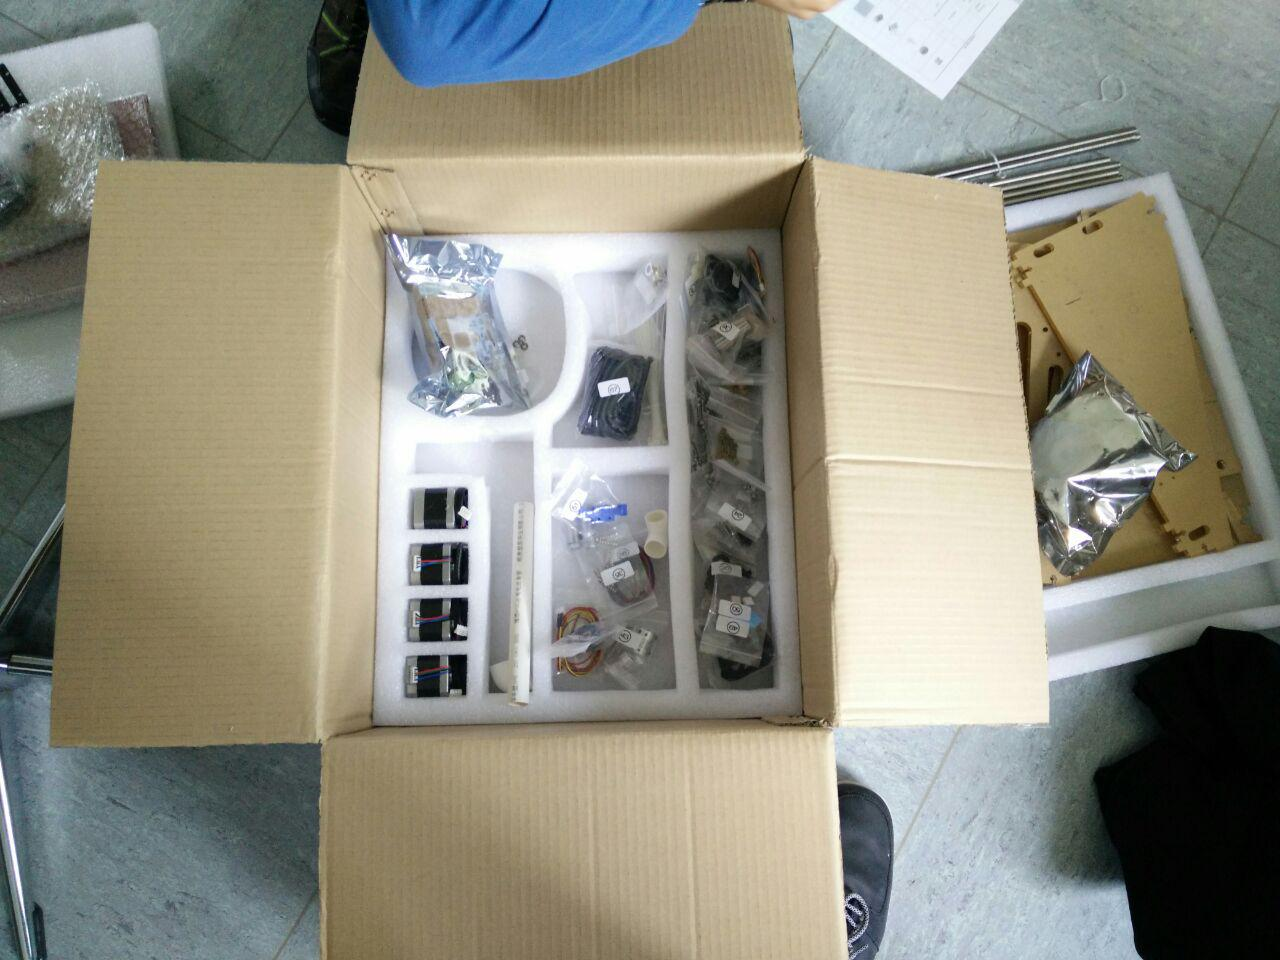
\includegraphics[clip=true,trim=230 100 320 100,angle=90,width=\textwidth]{Bilder/Material_1.jpg}
Enthalten hierin waren:
\begin{itemize}[noitemsep]
\item 4x NEMA17 Schrittmotoren
\item Die Kupplungen (Verbindungelemente zwischen Schrittmotor und Z-Achse)
\item GT2 Pulleys
\item X-Achen-Pulley-Verbinder (blaues Plastikteil)
\item Das GeeeTech GT2560 Steuerboard
\item Kabelbinder und Spiralschlauch
\item Lüfter und passende Kabel
\item Verschiedene Schrauben (M3)
\item Linearlager (8mm Innendurchmesser)
\item Teile für die Filamentrollenhalterung (Plastikrohre)
\end{itemize}
\vspace{\linewidth}
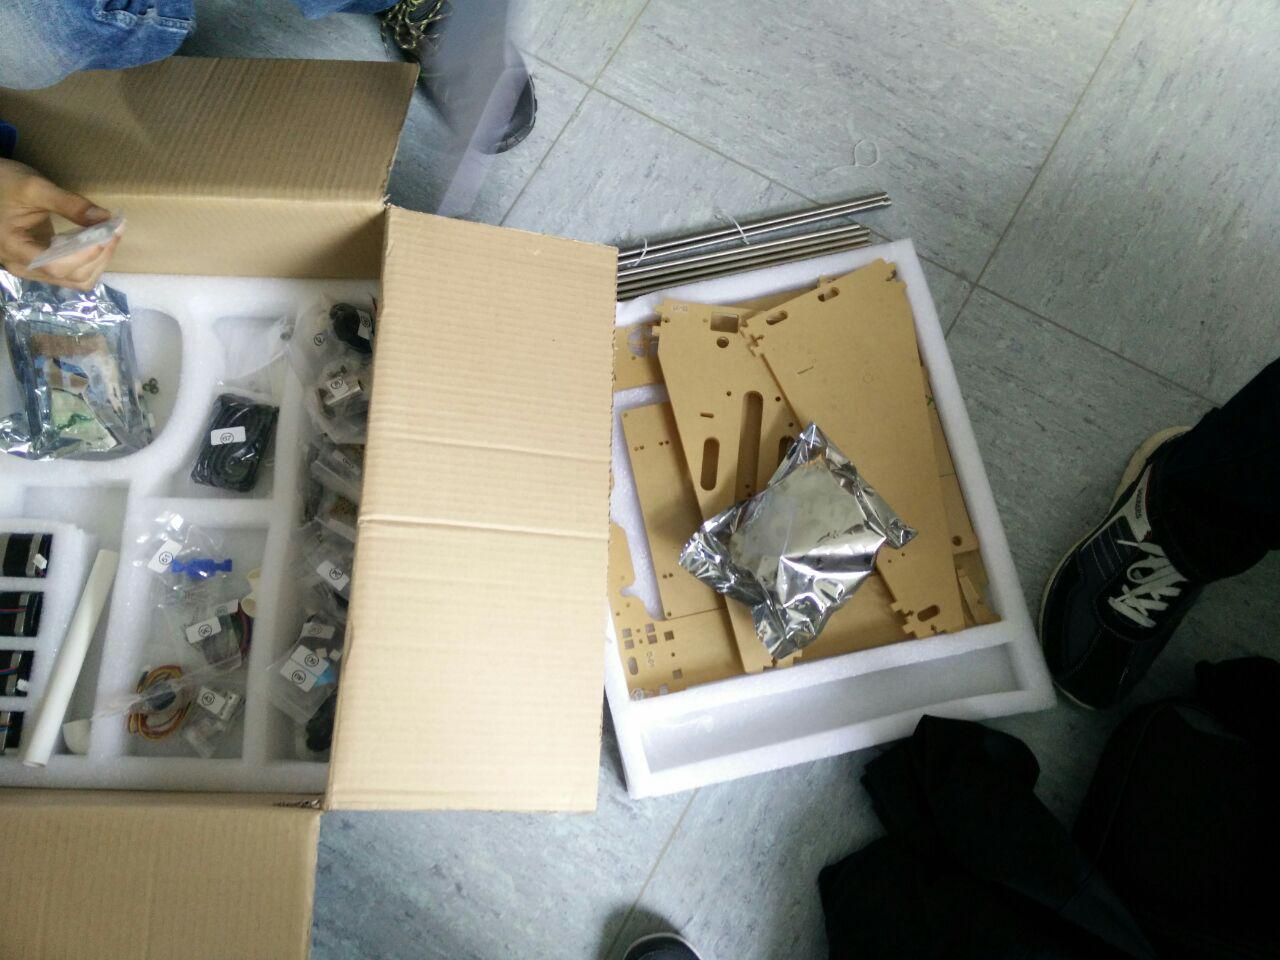
\includegraphics[clip=true,trim=410 100 150 100,angle=90,width=\textwidth]{Bilder/Material_2.jpg}
In dieser Packung enthalten waren:
\begin{itemize}[noitemsep]
\item Die verschiedenen Acryl-Platten
\subitem 4x Y-Achsen-Platten
\subitem XZ-Achsen-Frame
\subitem 2x XZ-Y-Verbinder-Platten
\subitem Heizbett-Platte
\subitem 2x Z-Achsen-Motor-Befestigungen
\subitem Die Platten des Filamentrollen-Halters
\subitem Sowie das LC-Display-Befestigungsmaterial

\item Die verschiedenen Linear-Stangen
\subitem Glatte Stahlstangen verschiedener Länge
\subitem 2x M8-Gewindestangen für die Z-Bewegung
\subitem 2x M8-Gewindestangen für den Y-Achsen-Aufbau
\end{itemize}
\vspace{\linewidth}
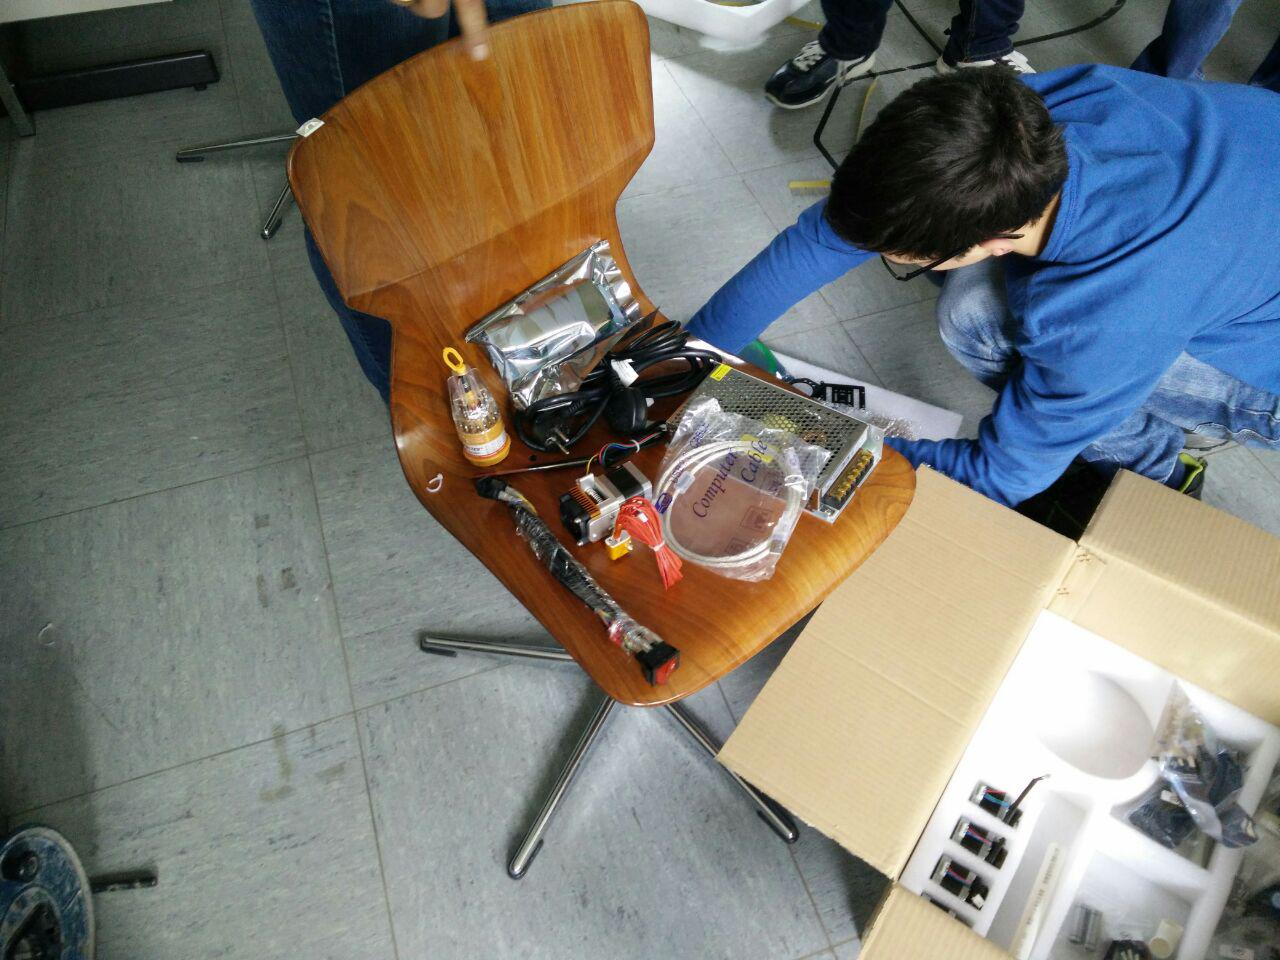
\includegraphics[clip=true,trim=260 180 230 160,width=\textwidth]{Bilder/Material_3.jpg}
Hier zu finden sind:
\begin{itemize}[noitemsep]
\item Das Netzteil, inklusive Stromkabel und Verbindungskabel mit Schalter
\item Den Extruder-Aufbau (mitsamt Motor, Hotend, Düse etc.)
\item Das Drucker LC-Display, über welches sich dieser steuern lässt, bzw. mit dessen Hilfe über SD-Karte gedruckt werden kann.
\item Das beiliegende Schraubendreher-Set
\item Das USB-Kabel zur Verbindung des GT2560 mit einem geeigneten Computer bzw. Pi
\item Einige Metallteile, z.B. die X-Schlitten-Platte
\end{itemize}

\newpage
\subsubsection{Schritt 1: Aufbau der Y-Achse}
Der obig verlinkten Anleitung folgend wurde beim Aufbau des Druckers zuerst die Y-Achse zusammen gebaut.
Hierfür wurden anfangs die nötigen Schrauben und Verbinder-Teile auf die zwei M8-Gewindestangen geschraubt:
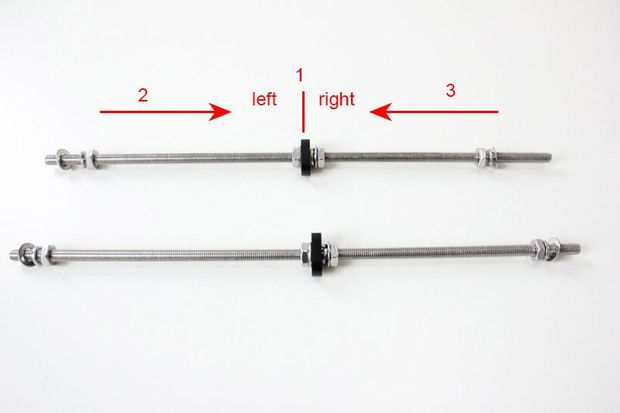
\includegraphics[clip=true,trim=0 100 0 40,width=\textwidth]{Bilder/Y_Assembly_Tutorial_1.jpg}

Als nächstes wurden die zwei Linear-Stangen zusammen mit den Y-Endplatten festgeschraubt. Wichtig ist, dass die Linearlager schon vorher auf die Stangen gesteckt werden!\\
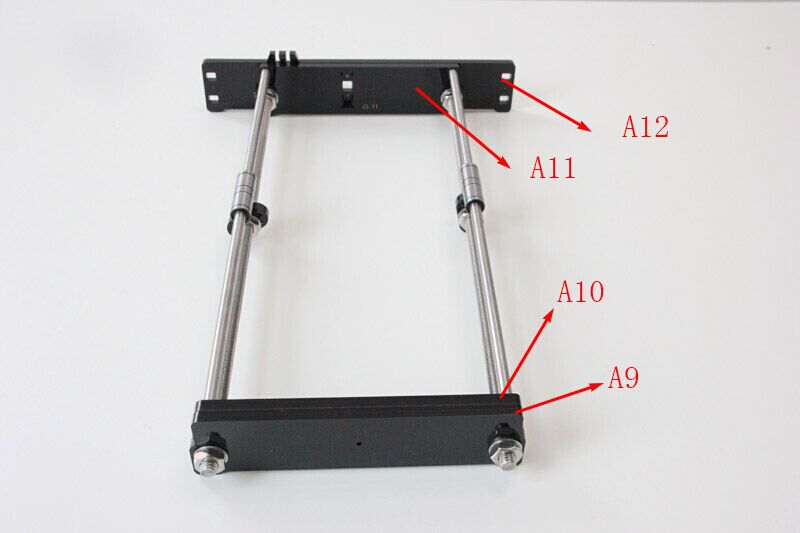
\includegraphics[width=\textwidth]{Bilder/Y_Assembly_Tutorial_2.jpg}
